\lstinputlisting[language=bash,basicstyle=\small]{python_codes/fieldstone_112/keywords}

\begin{center}
\inpython~Code at \url{https://github.com/cedrict/fieldstone/tree/master/python_codes/fieldstone_112}
\end{center}

\par\noindent\rule{\textwidth}{0.4pt}

%%%%%%%%%%%%%%%%%%%%%%%%%%%%%%%%%%%%%%%%%%%%%%%%%%%%%%%%%%%%%%%%%%%%%%%%%%%%%%%%%%%%%%%%%%%%%%%%%%%%

This \stone showcases the MINI (Section~\ref{pair:mini}), 
$P_2\times P_1$ (Section~\ref{ss:p2p1}), $Q_2\times Q_1$ (Section~\ref{ss:pairq2q1}), 
$Q_2\times P_{-1}$ (Section~\ref{ss:pairq2pm1} - unmapped approach, see \stone~76) 
and Crouzeix-Raviart  (Section~\ref{sec:crouzeix-raviart}) elements.

The mesh is composed of $nel_x \times nel_y$ cells which are cut in half via the same 
diagonal (NW-SE) into 2 triangles for simplicity when triangular elements are used: 

\begin{center}

\includegraphics[width=7cm]{python_codes/fieldstone_112/results/exp1/grid_quads}

\includegraphics[width=7cm]{python_codes/fieldstone_112/results/exp1/grid_triangles}\\
{\captionfont Quadrilaterals and triangles mesh for a resolution of $16\times 16$ cells.} 
\end{center}

A pressure dof is fixed so remove the nullspace and the obtained pressure field
is then normalised so that $\int_\Omega p dV = 0$.

Resolutions are ranging from 8x8 to 512x512. The high resolution runs take hours 
because python is slow. Most of what follows only goes up to 256x256. 320x320 seems 
to be the limit on my 32Gb-RAM laptop.  

\newpage
%========================================================
\subsection*{Donea \& Huerta manufactured solution}

We start with the manufactured solution problem "Donea \& Huerta" (see Section~\ref{mms1}).

\begin{center}
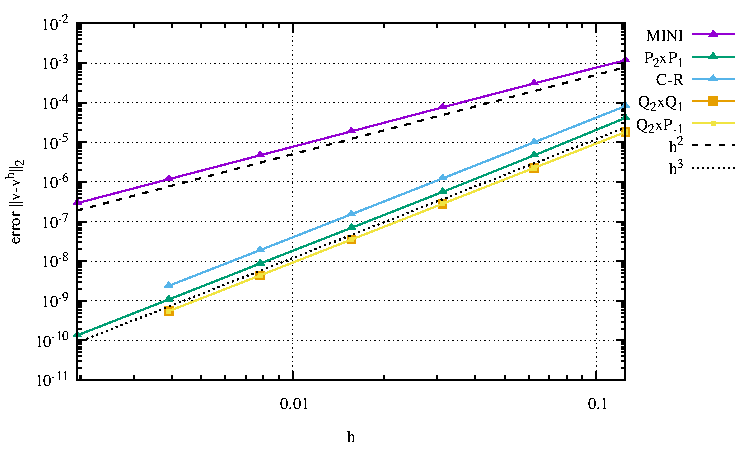
\includegraphics[width=8cm]{python_codes/fieldstone_112/results/exp1/errors_V.pdf}
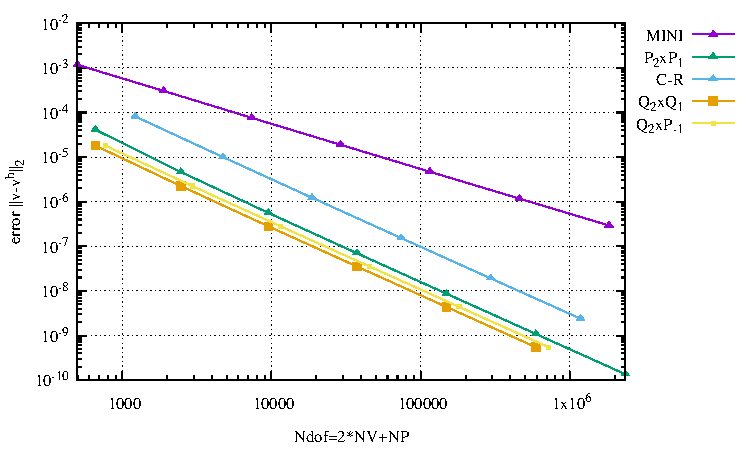
\includegraphics[width=8cm]{python_codes/fieldstone_112/results/exp1/errors_V_ndof.pdf}\\
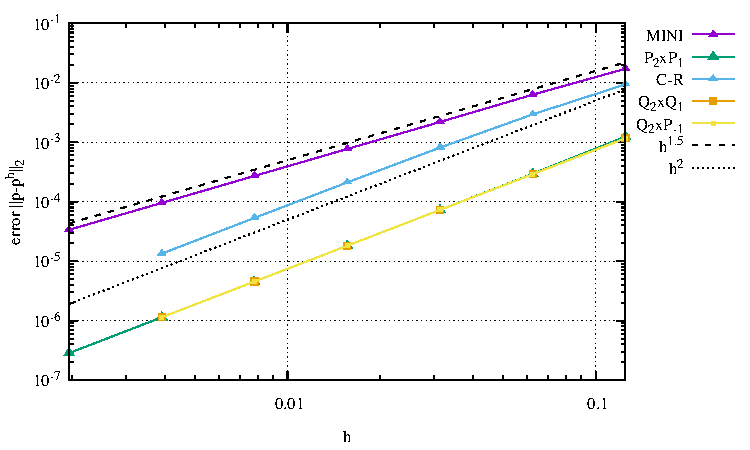
\includegraphics[width=8cm]{python_codes/fieldstone_112/results/exp1/errors_P.pdf}
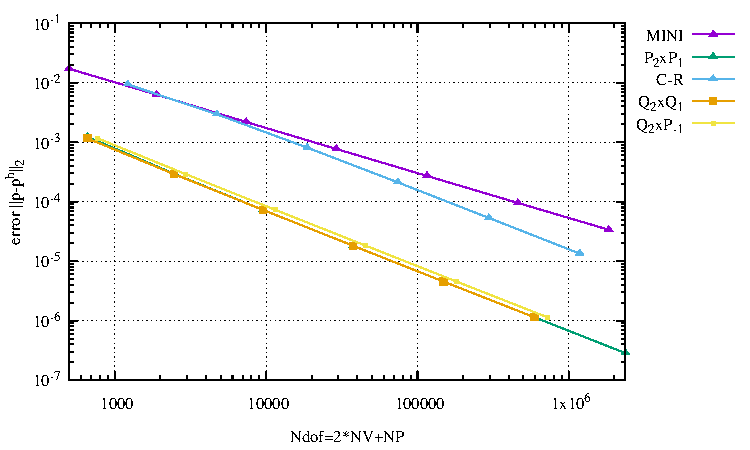
\includegraphics[width=8cm]{python_codes/fieldstone_112/results/exp1/errors_P_ndof.pdf}\\
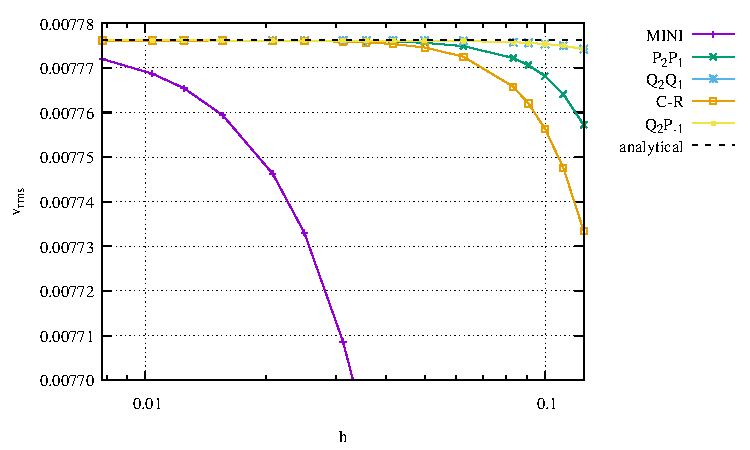
\includegraphics[width=8cm]{python_codes/fieldstone_112/results/exp1/vrms.pdf}
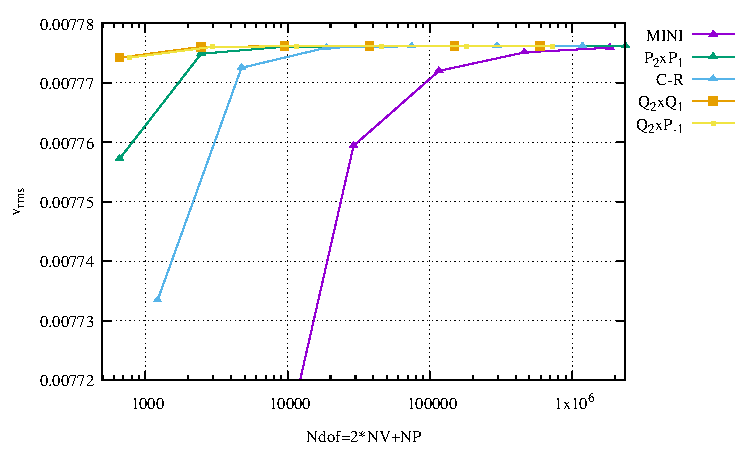
\includegraphics[width=8cm]{python_codes/fieldstone_112/results/exp1/vrms_ndof.pdf}\\
{\captionfont Velocity $L_2$ error (top row), pressure $L_2$ error (middle row) and root
mean square velocity (bottom row) as a function of the element size $h$ (left column) 
and the total number of degrees of freedom (right column).}
\end{center}

\newpage
\begin{center}
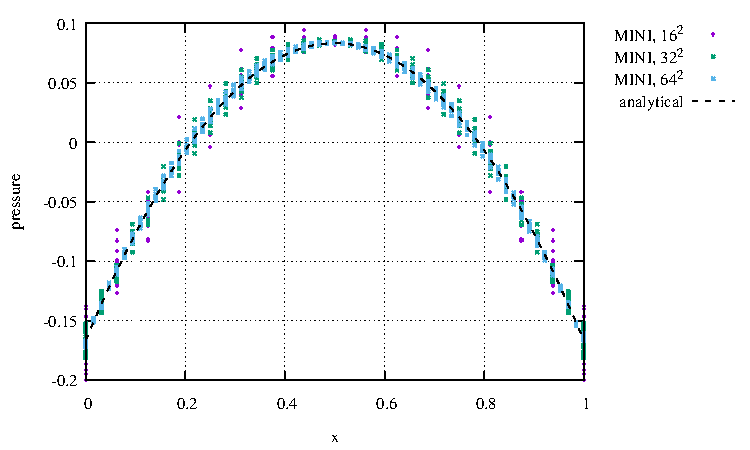
\includegraphics[width=8.5cm]{python_codes/fieldstone_112/results/exp1/pressMINI}
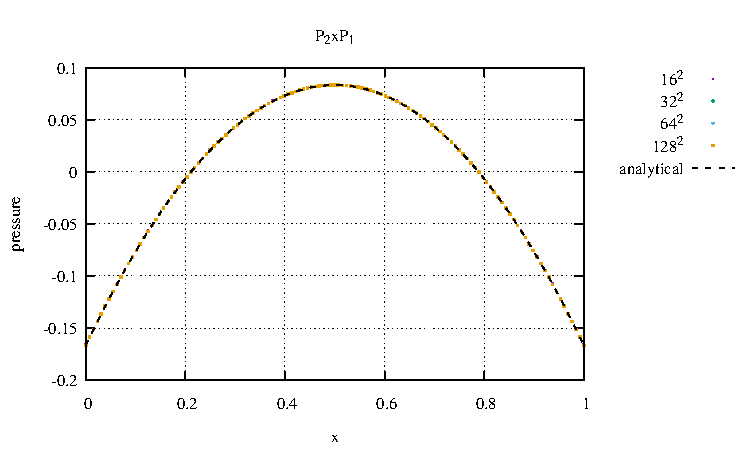
\includegraphics[width=8.5cm]{python_codes/fieldstone_112/results/exp1/pressP2P1}\\
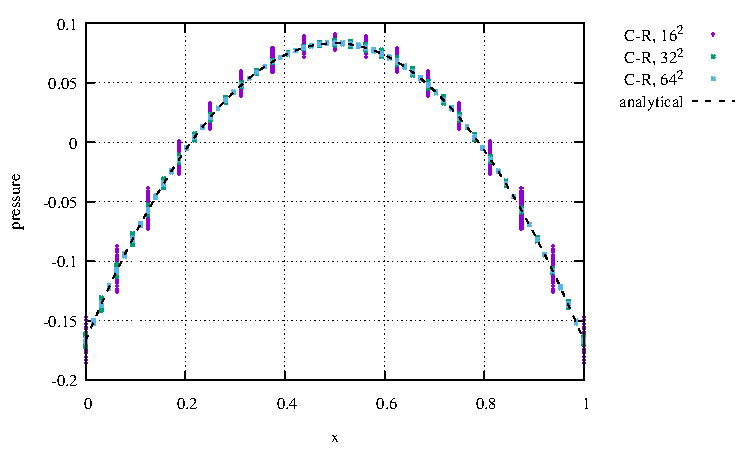
\includegraphics[width=8.5cm]{python_codes/fieldstone_112/results/exp1/pressCR}
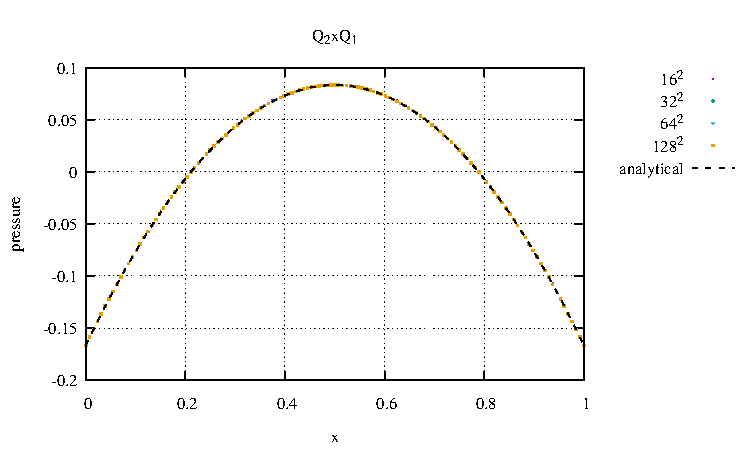
\includegraphics[width=8.5cm]{python_codes/fieldstone_112/results/exp1/pressQ2Q1}\\
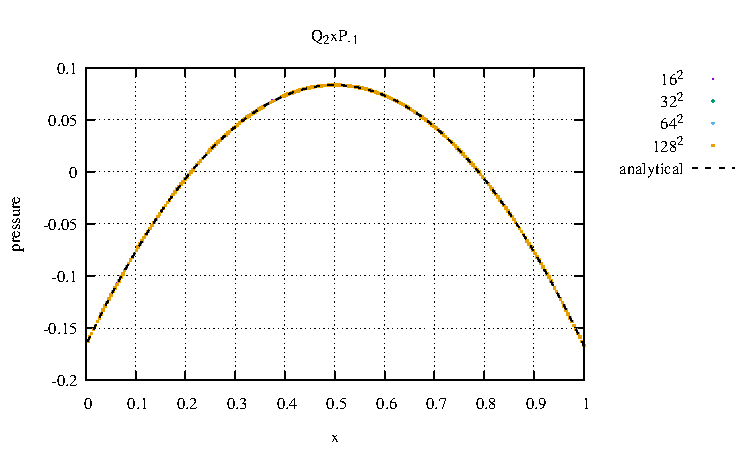
\includegraphics[width=8.5cm]{python_codes/fieldstone_112/results/exp1/pressQ2P1}\\
{\captionfont Pressure field as a function of the $x$-coordinate on a $16\times16$,
$32\times 32$ and $64\times 64$ mesh for all 5 elements.} 
\end{center}

\newpage

Influence of mesh quality:
A random perturbation is added to the interior nodes. 

\begin{center}
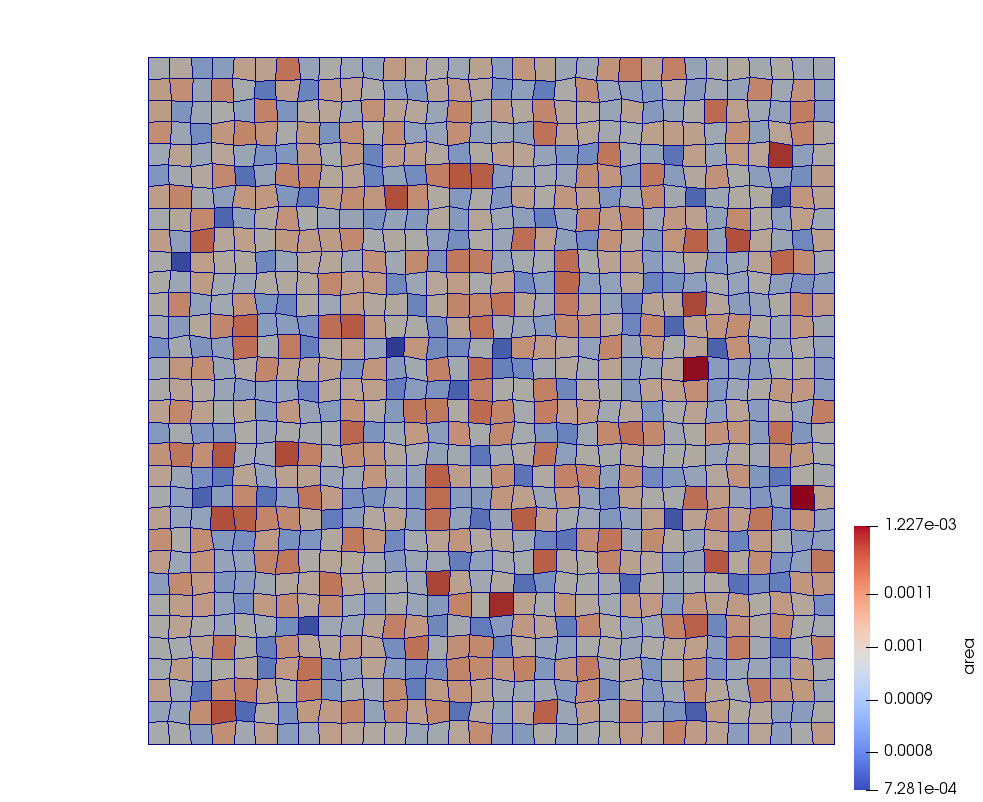
\includegraphics[width=6cm]{python_codes/fieldstone_112/results/exp1_rand/area_quads}
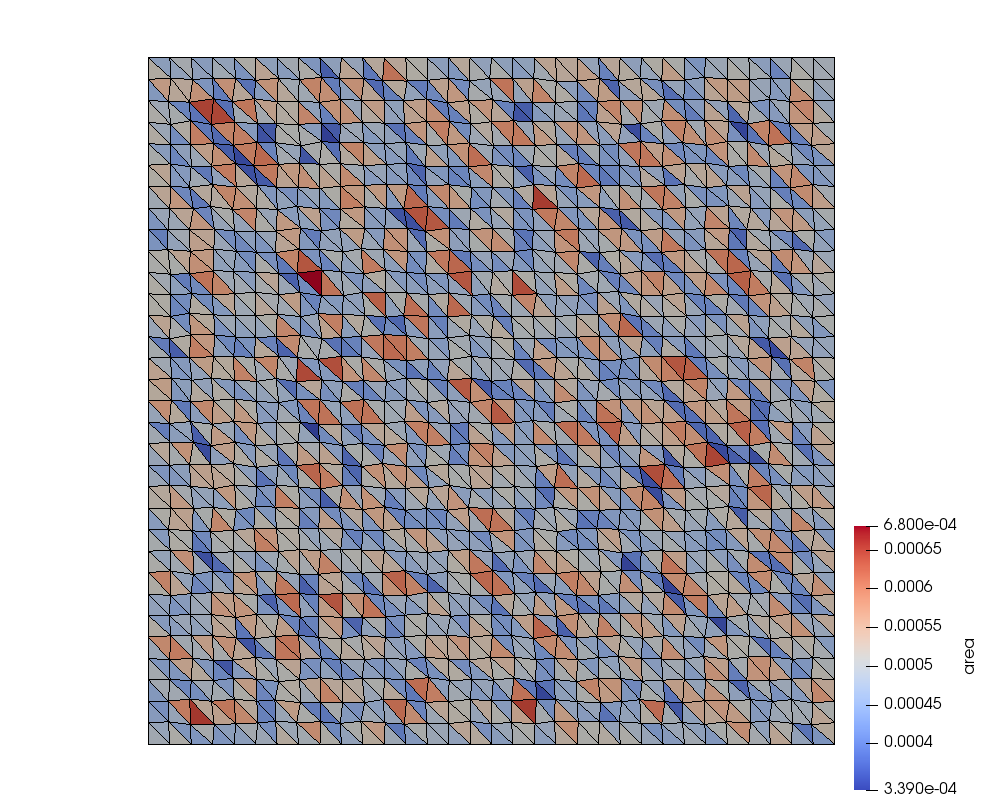
\includegraphics[width=6cm]{python_codes/fieldstone_112/results/exp1_rand/area_tris}\\
{\captionfont Mesh and element areas for quadrilaterals and triangles on a 32x32 cell mesh.}
\end{center}

\begin{center}
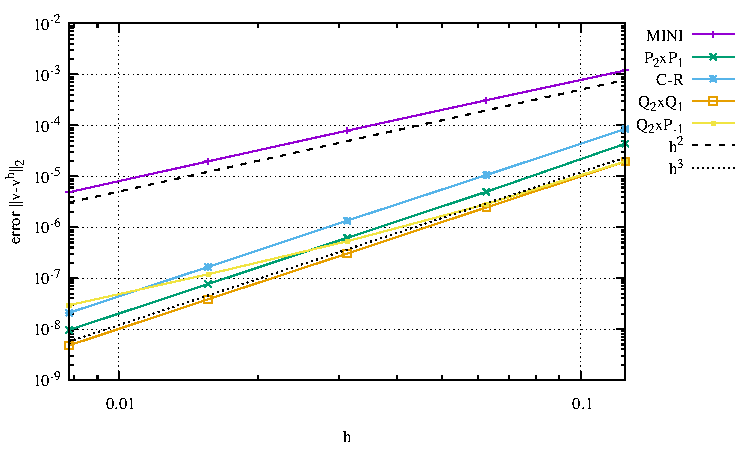
\includegraphics[width=8cm]{python_codes/fieldstone_112/results/exp1_rand/errors_V.pdf}
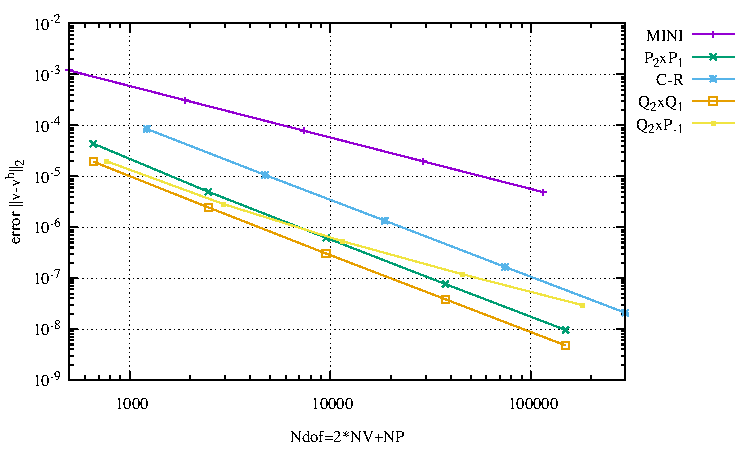
\includegraphics[width=8cm]{python_codes/fieldstone_112/results/exp1_rand/errors_V_ndof.pdf}\\
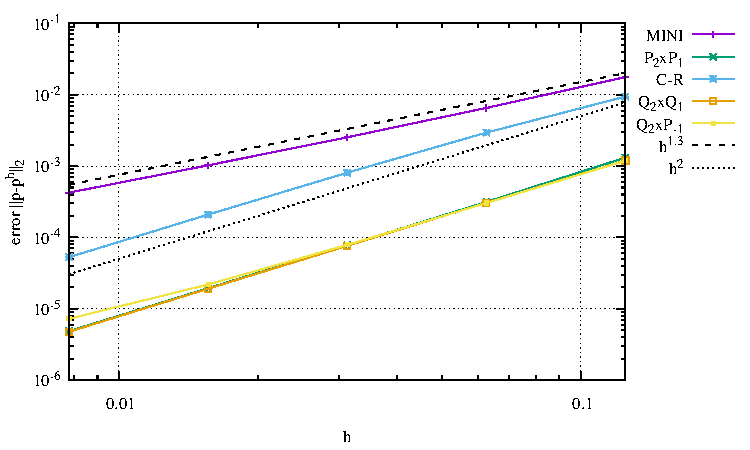
\includegraphics[width=8cm]{python_codes/fieldstone_112/results/exp1_rand/errors_P.pdf}
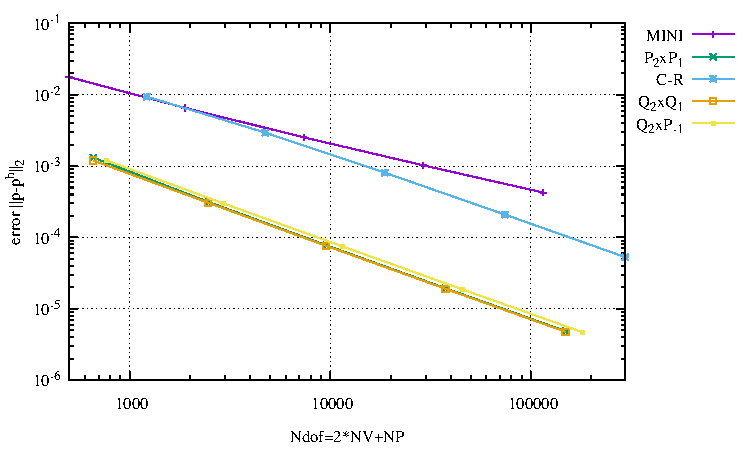
\includegraphics[width=8cm]{python_codes/fieldstone_112/results/exp1_rand/errors_P_ndof.pdf}\\
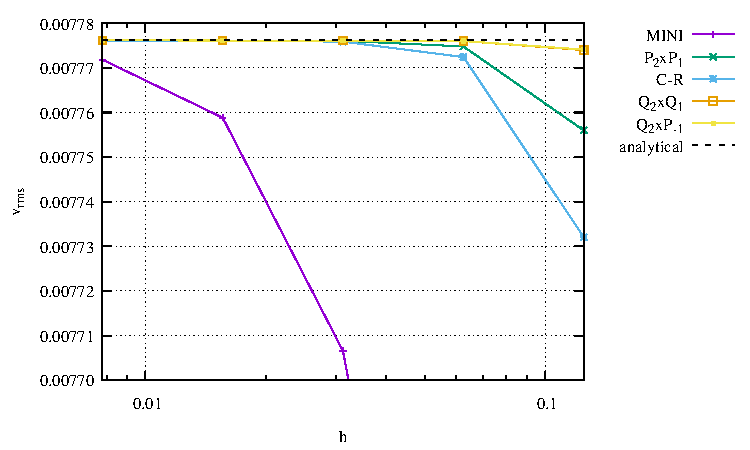
\includegraphics[width=8cm]{python_codes/fieldstone_112/results/exp1_rand/vrms.pdf}
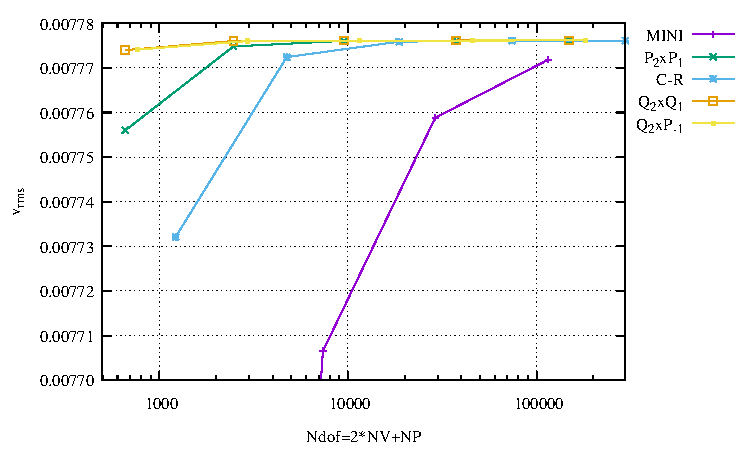
\includegraphics[width=8cm]{python_codes/fieldstone_112/results/exp1_rand/vrms_ndof.pdf}\\
{\captionfont Velocity $L_2$ error (top row), pressure $L_2$ error (middle row) and root
mean square velocity (bottom row) as a function of the element size $h$ (left column) 
and the total number of degrees of freedom (right column).}
\end{center}

\newpage
\begin{center}
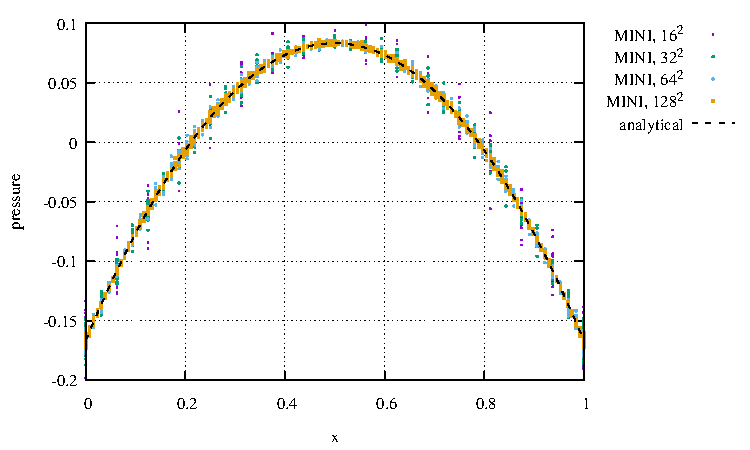
\includegraphics[width=8.5cm]{python_codes/fieldstone_112/results/exp1_rand/pressMINI}
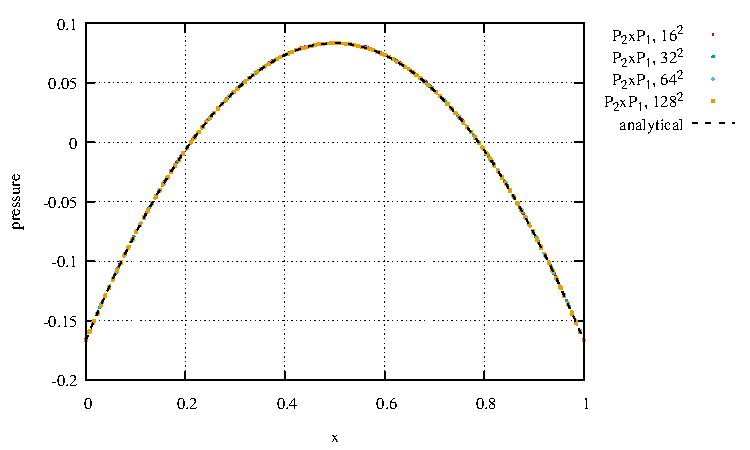
\includegraphics[width=8.5cm]{python_codes/fieldstone_112/results/exp1_rand/pressP2P1}\\
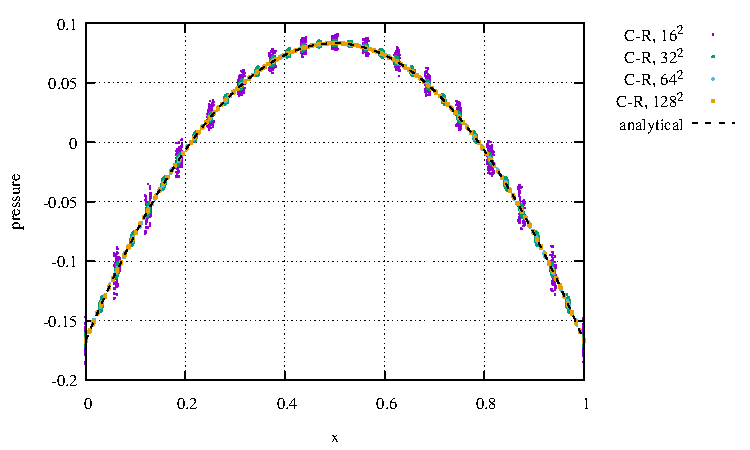
\includegraphics[width=8.5cm]{python_codes/fieldstone_112/results/exp1_rand/pressCR}
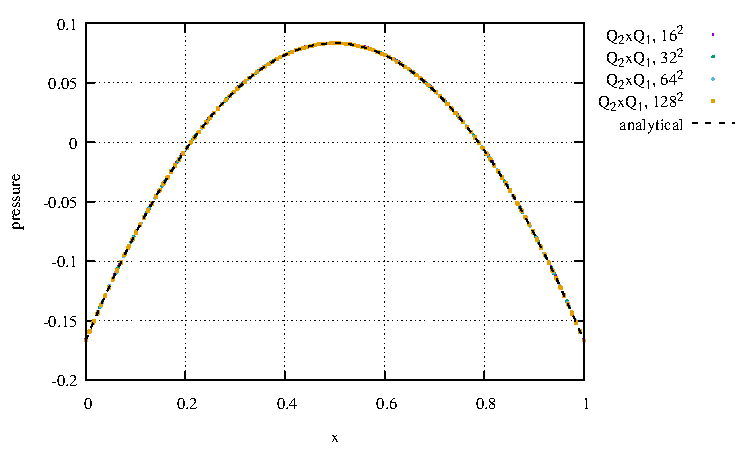
\includegraphics[width=8.5cm]{python_codes/fieldstone_112/results/exp1_rand/pressQ2Q1}\\
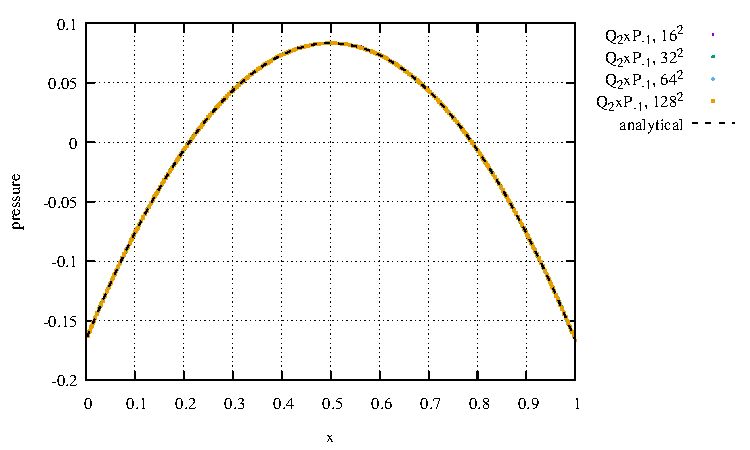
\includegraphics[width=8.5cm]{python_codes/fieldstone_112/results/exp1_rand/pressQ2P1}\\
{\captionfont Pressure field as a function of the $x$-coordinate on a $16\times16$,
$32\times 32$ and $64\times 64$ mesh for all 5 elements.} 
\end{center}

\newpage
%========================================================
\subsection*{Sinking block}

The setup is described in Section~\ref{ss:sinking_block}. No-slip boundary conditions case.
A sinker of size $0.125\times 0.125$ is placed in the middle of the domain. It has density
$\rho=1.01$ while the surrounding fluid has density $\rho=1$. Their respective viscosity is
$\eta=10^3$ and $\eta_1$. Gravity is vertical pointing downwards with $|\vec g|=1$.


\begin{center}
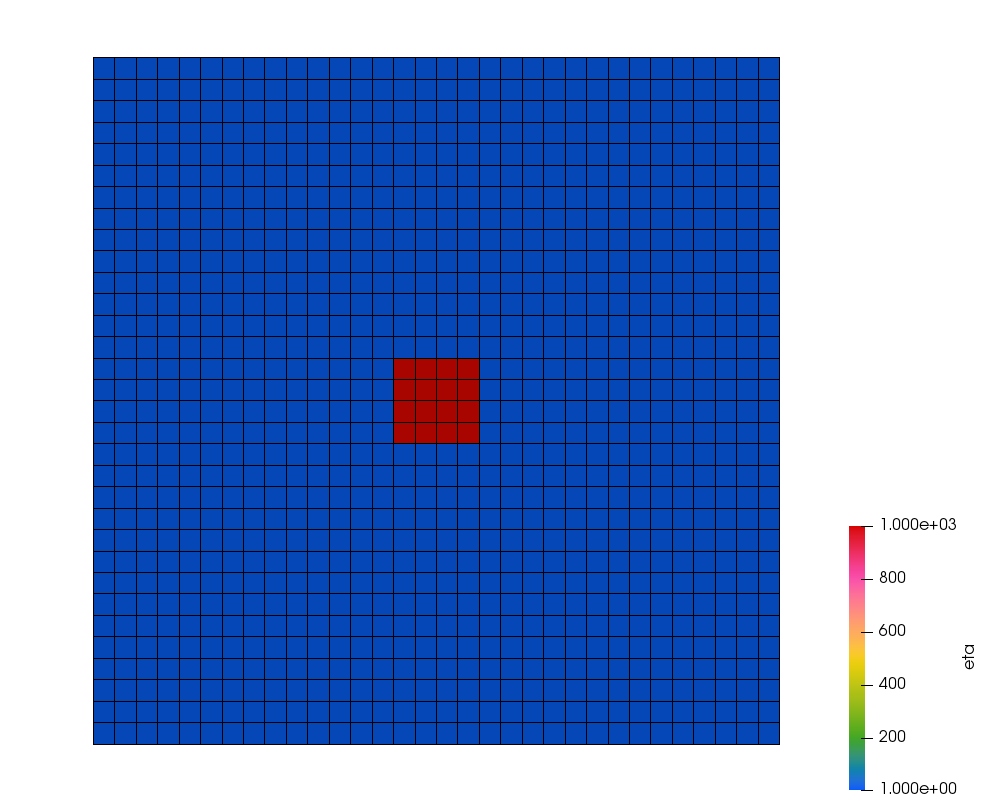
\includegraphics[width=8cm]{python_codes/fieldstone_112/results/exp2/eta}
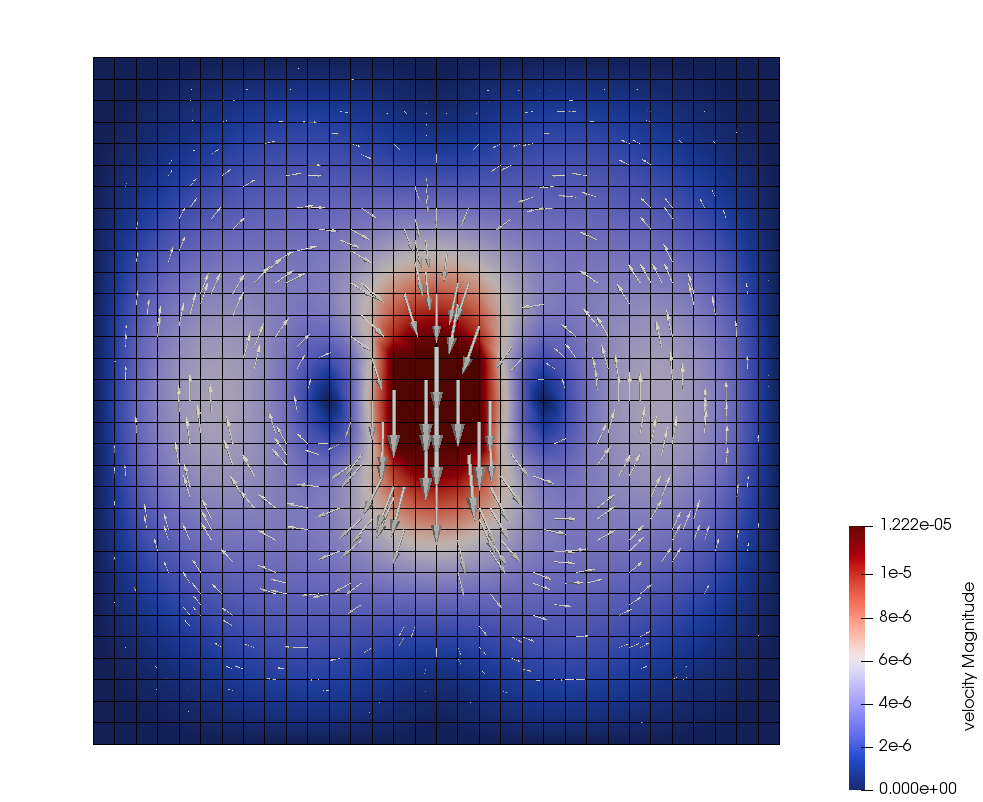
\includegraphics[width=8cm]{python_codes/fieldstone_112/results/exp2/vel}\\
{\captionfont $32\times 32$ grid, $Q_2\times P_{-1}$ element.}
\end{center}

We run this experiment on a $32\times 32$ cell mesh (these cells are then cut in half
in the case of triangular elements). Velocity and pressure are measured on two profiles,
one vertical and one horizontal passing through the middle of the domain.   

\begin{center}
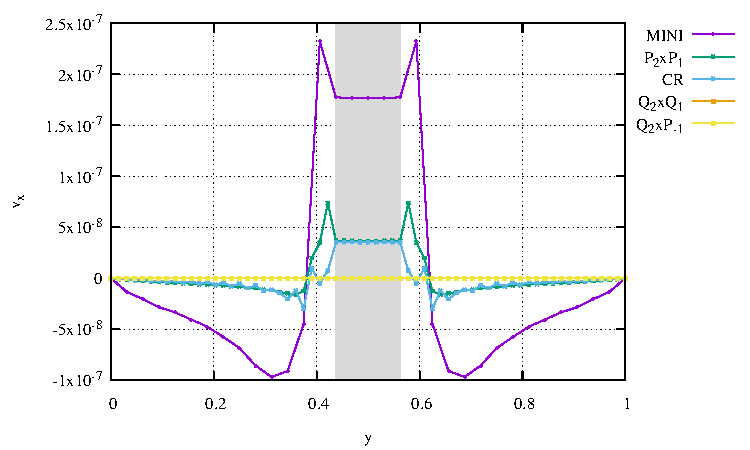
\includegraphics[width=8cm]{python_codes/fieldstone_112/results/exp2/vprofile_u.pdf}
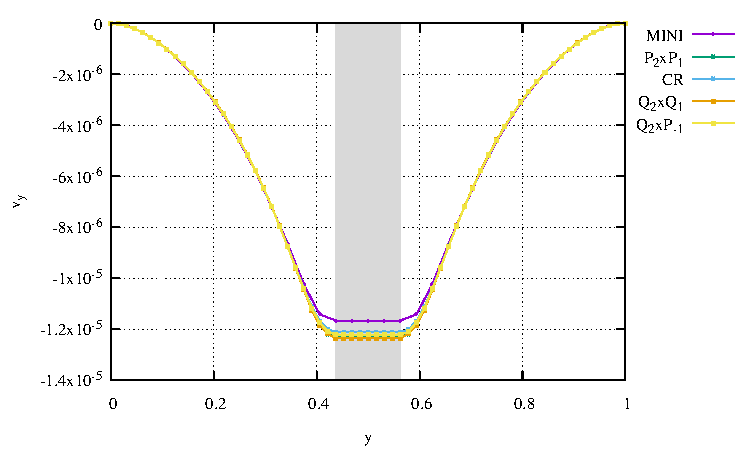
\includegraphics[width=8cm]{python_codes/fieldstone_112/results/exp2/vprofile_v.pdf}\\
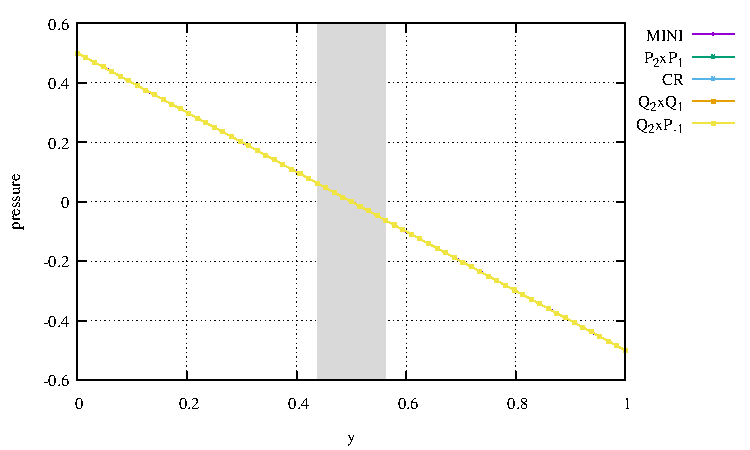
\includegraphics[width=8cm]{python_codes/fieldstone_112/results/exp2/vprofile_p.pdf}
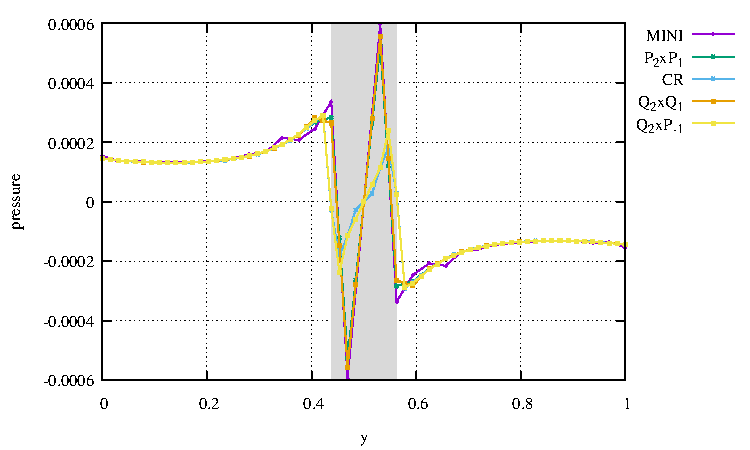
\includegraphics[width=8cm]{python_codes/fieldstone_112/results/exp2/vprofile_pdyn.pdf}\\
{\captionfont Vertical profiles. Pressure is projected onto the velocity nodes.}
\end{center}

\begin{center}
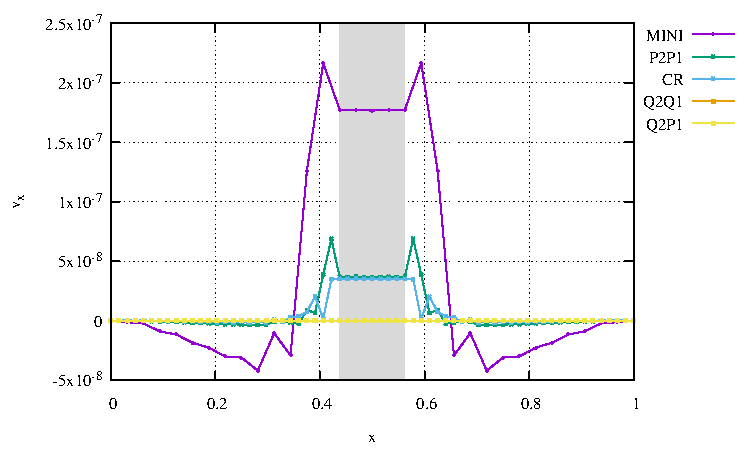
\includegraphics[width=8cm]{python_codes/fieldstone_112/results/exp2/hprofile_u.pdf}
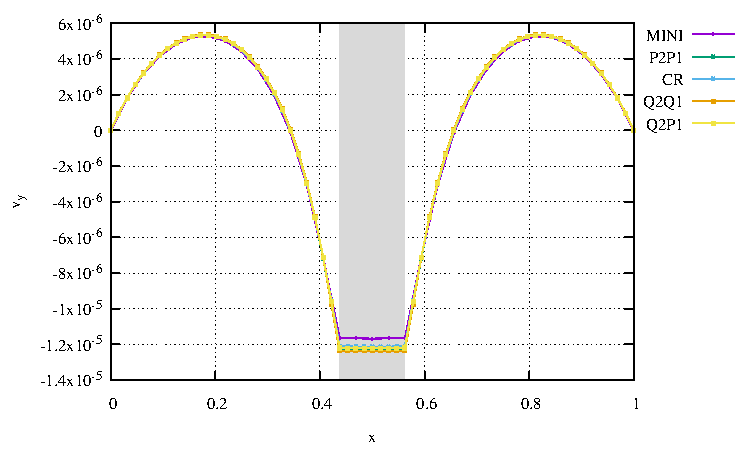
\includegraphics[width=8cm]{python_codes/fieldstone_112/results/exp2/hprofile_v.pdf}
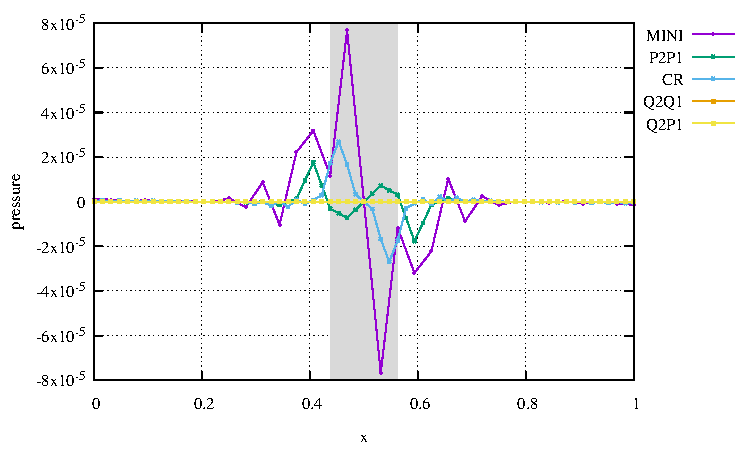
\includegraphics[width=8cm]{python_codes/fieldstone_112/results/exp2/hprofile_p.pdf}\\
{\captionfont Horizontal profiles. Pressure is projected onto the velocity nodes.}
\end{center}

\begin{center}
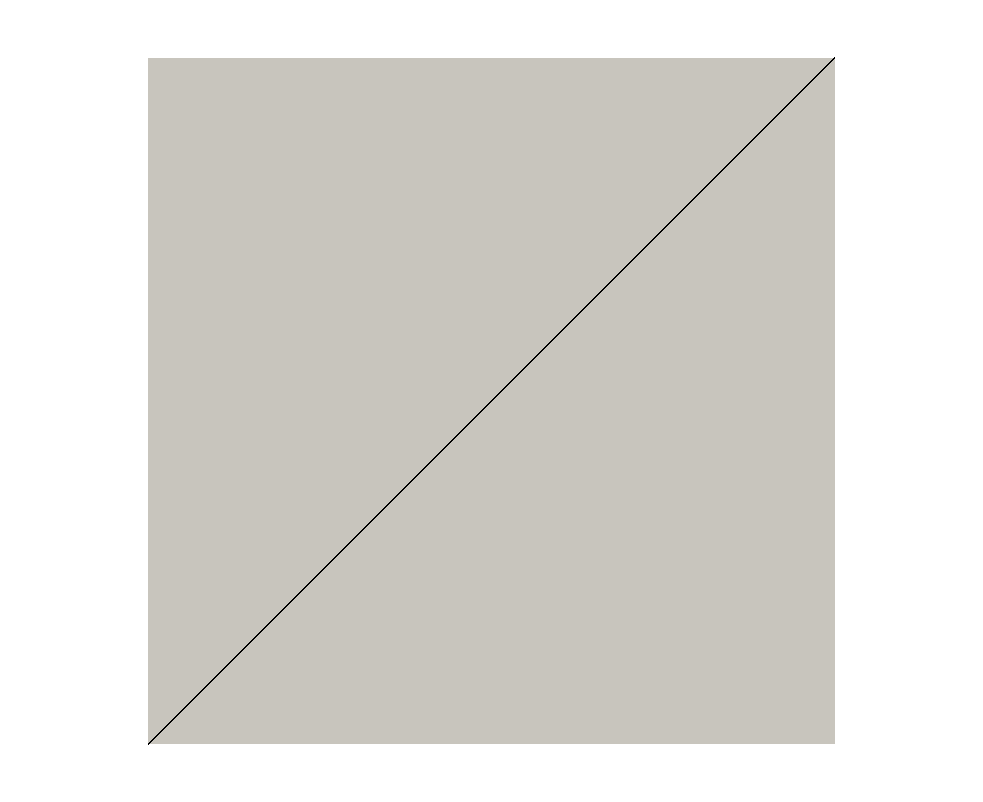
\includegraphics[height=6cm]{python_codes/fieldstone_112/results/exp2/diag.png}
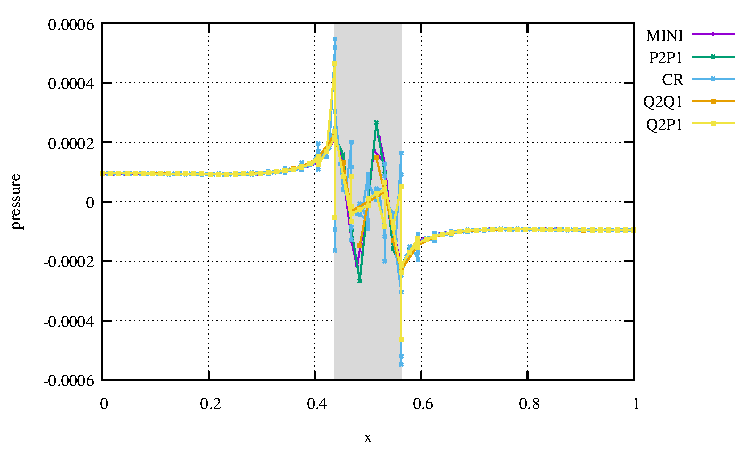
\includegraphics[height=6cm]{python_codes/fieldstone_112/results/exp2/diag_profile_p.pdf}\\
{\captionfont Dynamic pressure $p-p_{lith}$ field on SW-NE diagonal}
\end{center}


\begin{center}
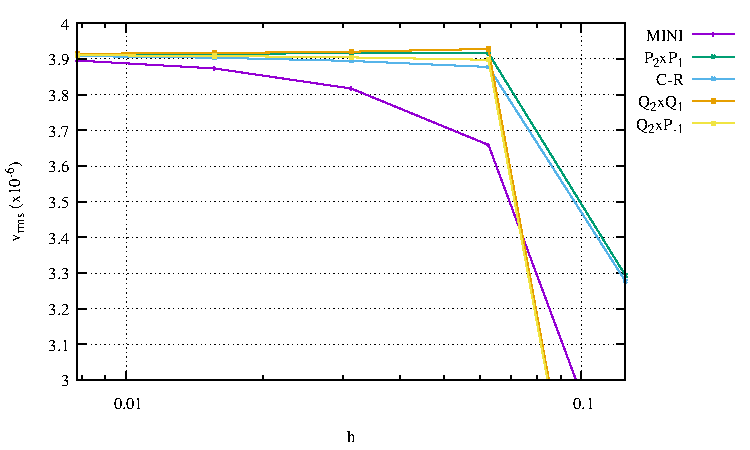
\includegraphics[width=8cm]{python_codes/fieldstone_112/results/exp2/vrms.pdf}
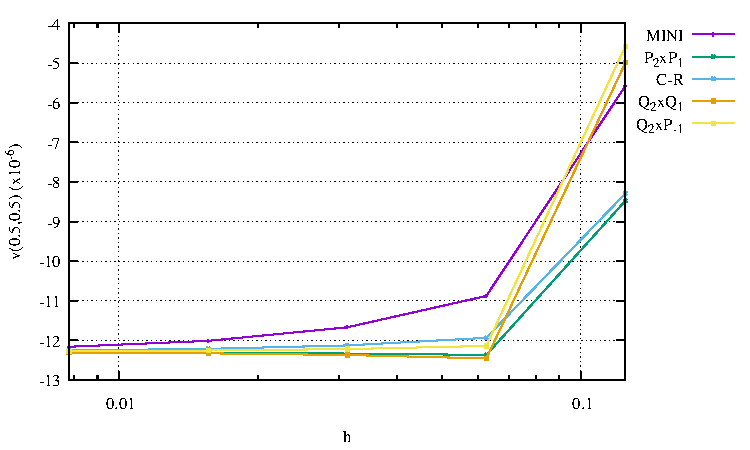
\includegraphics[width=8cm]{python_codes/fieldstone_112/results/exp2/v_center.pdf}\\
{\captionfont Left: root mean square velocity; Right: vertical velocity in the middle of the domain/sinker.}
\end{center}

\newpage
%========================================================
\subsection*{SolCx}

The setup is described in Section~\ref{ss:solcx}. The viscosity is discontinuous 
along the vertical line $x=1/2$ so discontinuous pressure elements perform better:

\begin{center}
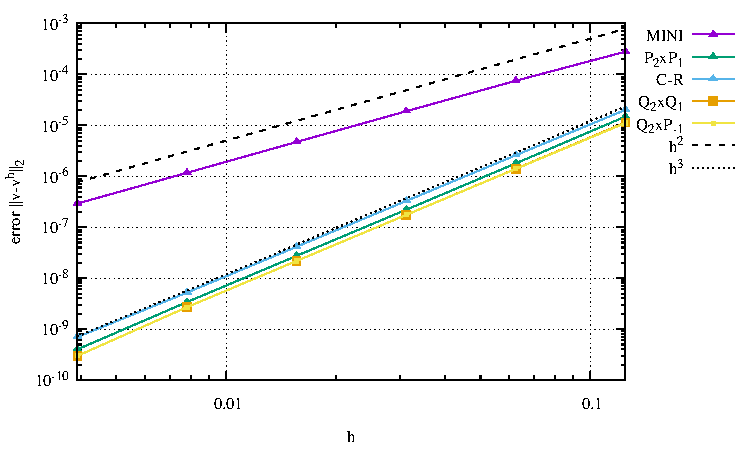
\includegraphics[width=8cm]{python_codes/fieldstone_112/results/exp3/errors_V.pdf}
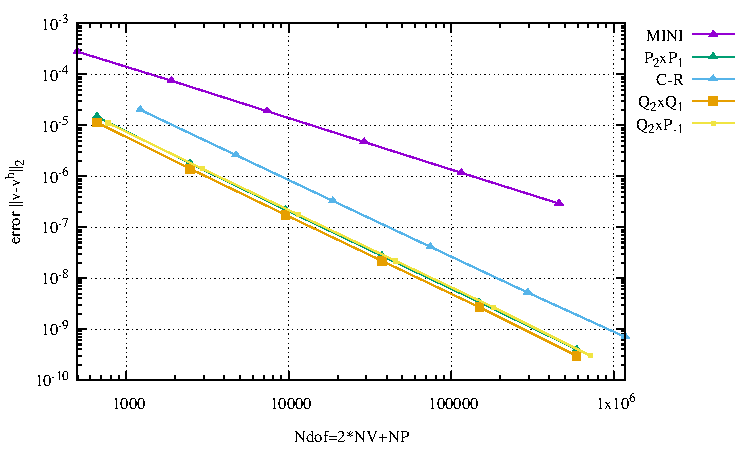
\includegraphics[width=8cm]{python_codes/fieldstone_112/results/exp3/errors_V_ndof.pdf}\\
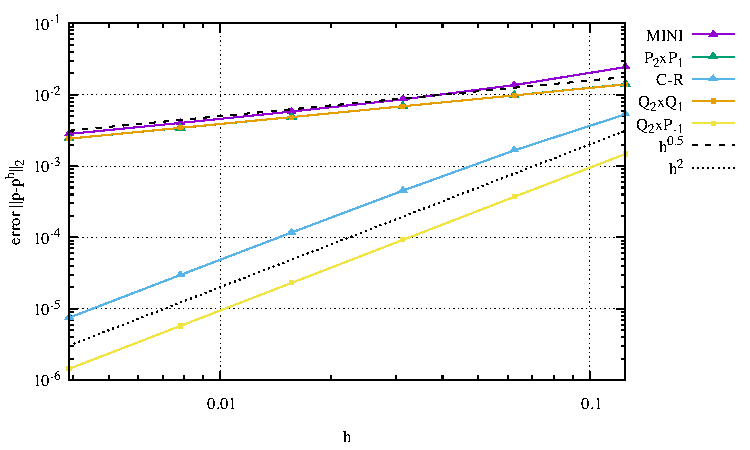
\includegraphics[width=8cm]{python_codes/fieldstone_112/results/exp3/errors_P.pdf}
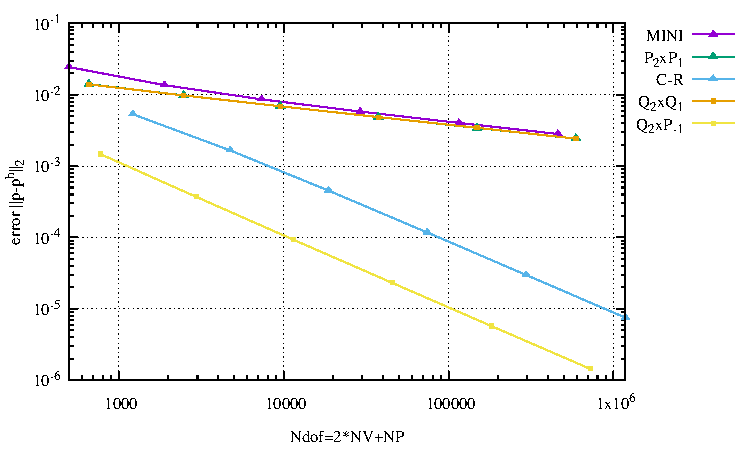
\includegraphics[width=8cm]{python_codes/fieldstone_112/results/exp3/errors_P_ndof.pdf}\\
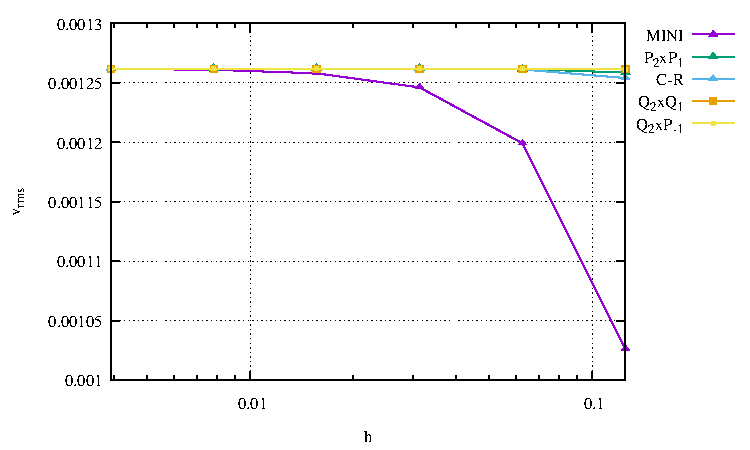
\includegraphics[width=8cm]{python_codes/fieldstone_112/results/exp3/vrms.pdf}
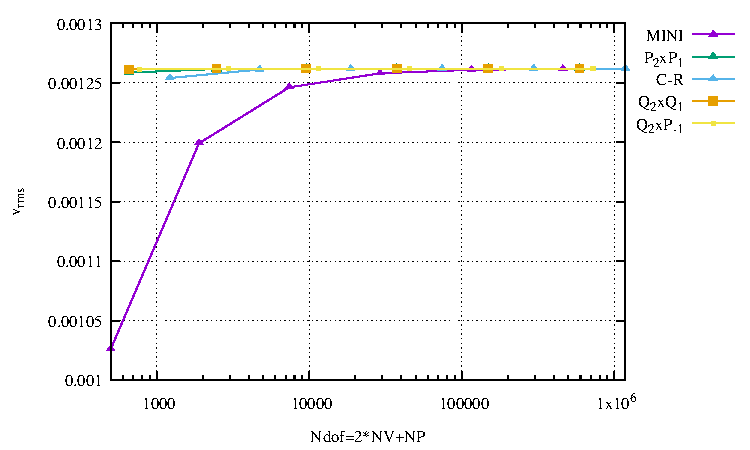
\includegraphics[width=8cm]{python_codes/fieldstone_112/results/exp3/vrms_ndof.pdf}\\
{\captionfont Velocity $L_2$ error (top row), pressure $L_2$ error (middle row) and vrms (bottom row) 
as a function of the element size $h$ (left column) and the total number of dofs (right column).}
\end{center}

Thieulot \& Bangerth (2021) \cite{thba21} report ${\cal O}(h^3)$ for velocity for both $Q_2\times Q_1$ and $Q_2\times P_1$
and ${\cal O}(h^{0.5})$ for $Q_2\times Q_1$ and  ${\cal O}(h^{2})$ for $Q_2\times P_{-1}$ for pressure. 
Our measurements are similar here.

\newpage
%========================================================
\subsection*{SolKz}

The setup is described in Section~\ref{ss:solkz}. 

\begin{center}
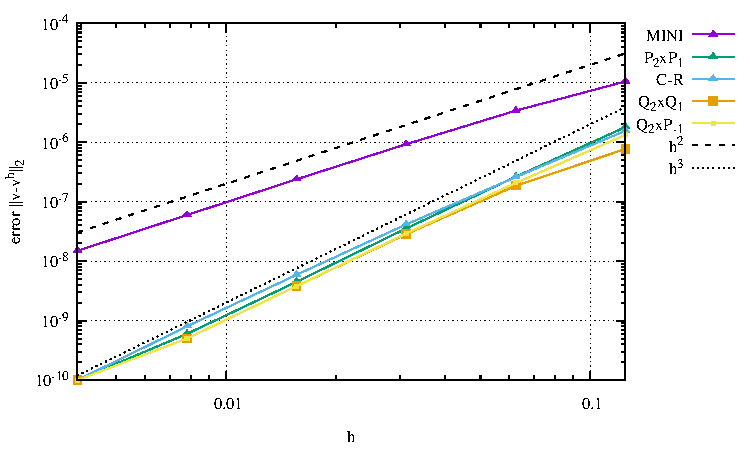
\includegraphics[width=8cm]{python_codes/fieldstone_112/results/exp4/errors_V.pdf}
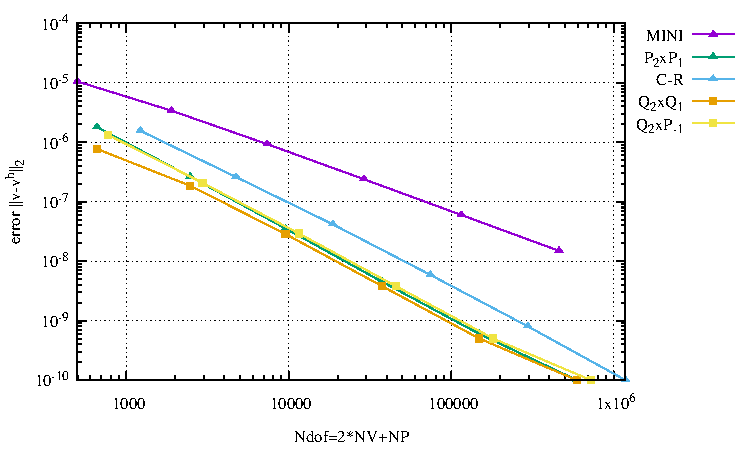
\includegraphics[width=8cm]{python_codes/fieldstone_112/results/exp4/errors_V_ndof.pdf}\\
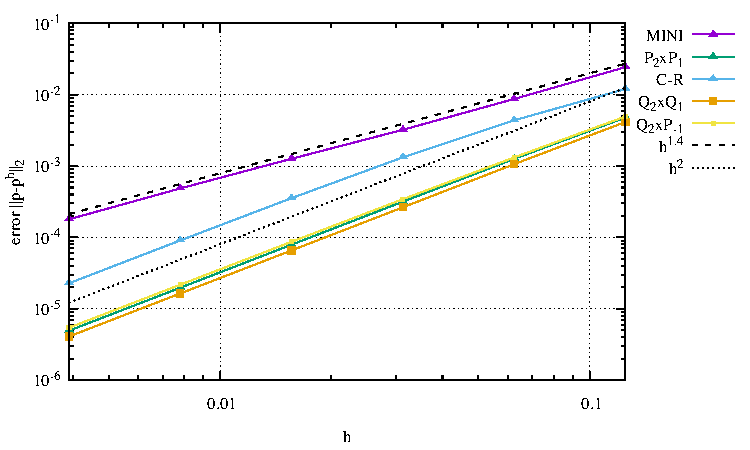
\includegraphics[width=8cm]{python_codes/fieldstone_112/results/exp4/errors_P.pdf}
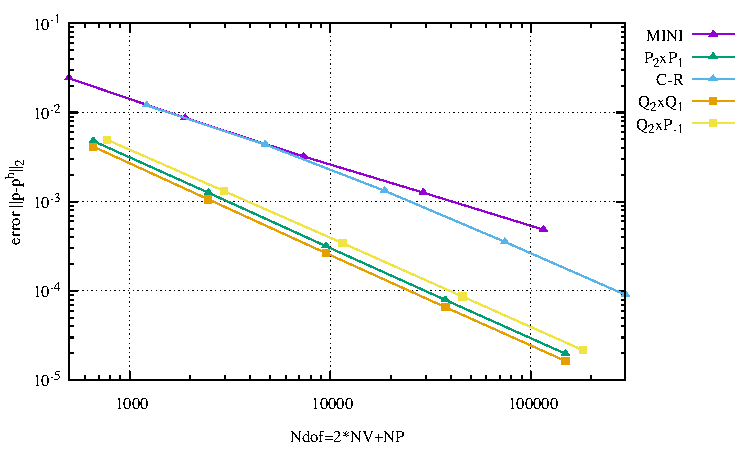
\includegraphics[width=8cm]{python_codes/fieldstone_112/results/exp4/errors_P_ndof.pdf}\\
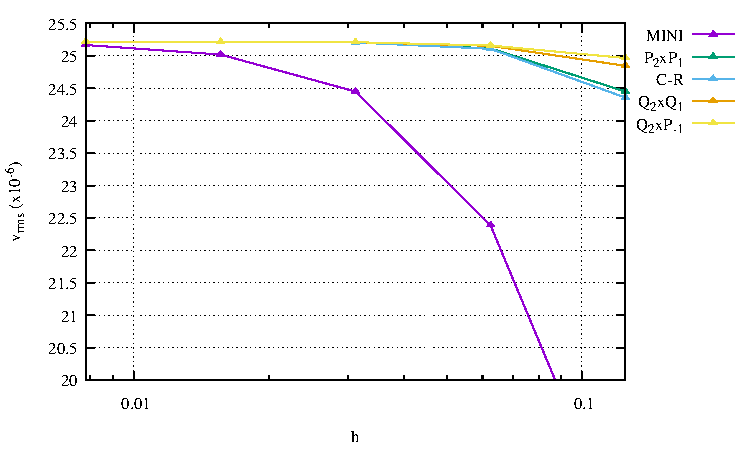
\includegraphics[width=8cm]{python_codes/fieldstone_112/results/exp4/vrms.pdf}
\includegraphics[width=8cm]{python_codes/fieldstone_112/results/exp4/vrms_ndof.pdf}\\
{\captionfont Velocity $L_2$ error (top row), pressure $L_2$ error (middle row) and vrms (bottom row) 
as a function of the element size $h$ (left column) and the total number of dofs (right column).}
\end{center}

Note the 1.4 convergence of pressure for MINI

\newpage
Influence of mesh quality: A random perturbation is added to the interior nodes. 

\begin{center}
\includegraphics[width=8cm]{python_codes/fieldstone_112/results/exp4_rand/errors_V.pdf}
\includegraphics[width=8cm]{python_codes/fieldstone_112/results/exp4_rand/errors_V_ndof.pdf}\\
\includegraphics[width=8cm]{python_codes/fieldstone_112/results/exp4_rand/errors_P.pdf}
\includegraphics[width=8cm]{python_codes/fieldstone_112/results/exp4_rand/errors_P_ndof.pdf}\\
\includegraphics[width=8cm]{python_codes/fieldstone_112/results/exp4_rand/vrms.pdf}
\includegraphics[width=8cm]{python_codes/fieldstone_112/results/exp4_rand/vrms_ndof.pdf}\\
{\captionfont Velocity $L_2$ error (top row), pressure $L_2$ error (middle row) and root
mean square velocity (bottom row) as a function of the element size $h$ (left column) 
and the total number of degrees of freedom (right column).}
\end{center}





\newpage
%========================================================
\subsection*{SolVi}

The setup is described in Section~\ref{ss:solvi}. 

\begin{center}
\includegraphics[width=8cm]{python_codes/fieldstone_112/results/exp5/errors_V.pdf}
\includegraphics[width=8cm]{python_codes/fieldstone_112/results/exp5/errors_V_ndof.pdf}\\
\includegraphics[width=8cm]{python_codes/fieldstone_112/results/exp5/errors_P.pdf}
\includegraphics[width=8cm]{python_codes/fieldstone_112/results/exp5/errors_P_ndof.pdf}\\
\includegraphics[width=8cm]{python_codes/fieldstone_112/results/exp5/vrms.pdf}
\includegraphics[width=8cm]{python_codes/fieldstone_112/results/exp5/vrms_ndof.pdf}\\
{\captionfont Velocity $L_2$ error (top row), pressure $L_2$ error (middle row) and vrms (bottom row) 
as a function of the element size $h$ (left column) and the total number of dofs (right column).}
\end{center}

Thieulot \& Bangerth (2021) \cite{thba21} report ${\cal O}(h)$ convergence for 
velocity and ${\cal O}(h^{0.5})$ for pressure across all four elements that they tested.
Our measurements are similar here.


\begin{center}
\includegraphics[width=8.5cm]{python_codes/fieldstone_112/results/exp5/bottom64}
\includegraphics[width=8.5cm]{python_codes/fieldstone_112/results/exp5/bottom128}\\
{\captionfont Pressure at the bottom of the domain. Grey area corresponds to the 
high viscosity disc. Left: 64x64 cells; right: 128x128 cells.}
\end{center}


\newpage




Assuming that $
\| {\bm u} - {\bm u}_h \|_{L_2} = {\cal O}(h^{\alpha_v})
$ and $
\| p - p_h \|_{L_2} = {\cal O}(h^{\alpha_p})
$
I have gathered the exponent values in the following 
table. 


\begin{tabular}{|l|llll|llll|llll|llll|llll|}
\hline
& 
\multicolumn{4}{c|}{MINI}&  
\multicolumn{4}{c|}{$P_2\times P_1$}  & 
\multicolumn{4}{c|}{C-R}  & 
\multicolumn{4}{c|}{$Q_2\times Q_1$} &  
\multicolumn{4}{c|}{$Q_2\times P_1$}  \\
experiment      & 
$\alpha_v$ & r  &  $\alpha_p$ & r &  
$\alpha_v$ & r  &  $\alpha_p$ & r &  
$\alpha_v$ & r  &  $\alpha_p$ & r &  
$\alpha_v$ & r  & $\alpha_p$ & r &   
$\alpha_v$ & r  & $\alpha_p$ & r \\
\hline
\hline
D \& H 
&{2}&4&1.5&3
&{3}&2&2&1
&{3}&3&2&2
&{3}&1&2&1
&{3}&1&2&1\\
D \& H (rand)
&2&5&1.3&3
&3&2&2&1
&3&3&2&2
&3&1&2&1
&3&1&2&1 \\
SolCx 
&2&4&0.5&4
&3&2&0.5&3
&3&3&2&2
&3&1&0.5&3
&3&1&2&1\\
SolKz 
&2&4&1.4&5
&3&2&2&2
&3&3&2&4
&3&1&2&1
&3&1&2&3\\
SolKz (rand)
&2&4&1.2&5
&3&2&2&2
&3&3&2&4
&3&1&2&1
&3&1&2&3\\
SolVi 
&1&-&0.5&3
&1&-&0.5&1
&1&-&0.5&4
&1&-&0.5&2
&1&-&0.5&5\\
\hline
total  
&-&17&-&16
&-&8&-&7
&-&12&-&12
&-&4&-&6
&-&?&-&?\\
\hline
\end{tabular}

The r value corresponds to the \textbf{r}anking. For instance if Q2Q1 is the most accurate for velocity on D \& H then it gets a 1, then P2P1 gets a 2 because it was the second best accurate element, etc ...
In the end I would sum all the r values per column 
and the smaller the value the better the element. 

Note that SolVi measurements will be updated when the 512x512 runs have completed so for now Solvi is not 
taken into account.

%========================================================
\subsection*{Preliminary Conclusions}

\begin{itemize}
\item the MINI element is very appealing (a single bubble added to $P_1$) and cheap. However it is also 
the least accurate element, even looking at the errors as function of number of dofs and not $h$
\item P2P1 always more accurate than CR except for SolCx where disc pressure elements are way more accurate.
\item P2P1 about as accurate as Q2Q1 in all benchmarks
\end{itemize}



%========================================================
\subsection*{Open questions}

\begin{itemize}
%\item what is a good measure $h$ for triangles in general ? sqrt of area ? hypothenuse ? min of edges length? 
\item at the moment I build the entire Stokes matrix in a sparse format and send it to the default 
python solver. This means that no iterative solver is used (inner or outer) so that the discussion 
on the nb of FGMRES iterations of our paper cannot be carried out here. 
\item Right now viscosity is computed on quadrature point. No averaging. It probably only really matters 
for SolVi (and may be a bit for SolKz). Should I implement elemental averaging and try?  
\item are there other elements you wish to add to this list? $P_3\times P_2$ ? 
\item should I better randomize the triangles by alternating the quadrilateral diagonals (SW-NE and NW-SE)?
\item I plot now the velocity and pressure errors as a function of the total number of dofs. Does this make sense? or should I 
plot the velocity errors as a fct of the velocity dofs and the pressure errors  as a fct of pressure dofs?
\item any thoughts about my ranking system ?like it ? hate it ?
\end{itemize}


note to myself: check and probably remove stone 46, 47 ?
